% ==========================================================================================
% Dissertation template and document class for Princeton University
% Author  : Jeffrey Scott Dwoskin <jdwoskin@princeton.edu>
% Adapted from: http://www.math.princeton.edu/graduate/tex/puthesis.html
% ==========================================================================================

%%-- For print copies
%% set 'singlespace' option to set entire thesis to single space, and define "\printmode" to remove all hyperlinks for printed copies of the thesis. Delete all output files before changing this mode -- it will turn hyperref package on and off
%\documentclass[12pt,lot, lof, singlespace]{puthesis}
%\newcommand{\printmode}{}

%%-- For the electronic copy, use doublespacing, define "\proquestmode" to use outlined links, instead of colored links.
\documentclass[12pt,lot, lof]{puthesis}
\newcommand{\proquestmode}{}
% I prefer proquestmode to be off for electronic copies for normal use, since the colored links are less distracting. However when printed in black and white, the colored links are difficult to read.

%%-- For early drafts without some of the frontmatter
% Also see the "ifodd" command below to disable more frontmatter
%\documentclass[12pt]{puthesis}

%%---- Author & title page info ----%%
\title{Recombination X-Ray Laser Based on Ionization-recombination Mechanism of Atomic Excitation}

\submitted{July 2011}  % degree conferral date (January, April, June, September, or November)
\copyrightyear{2011}  % year in which the copyright is secured by publication of the dissertation.
\author{Chao LU}
\adviser{Professor Marlan O. Scully}  %replace with the full name of your adviser
%\departmentprefix{Program in}  % defaults to "Department of", but programs need to change this.
\department{Mechanical Engineering}

%%---- Tweak float placements ----%%
% From: http://mintaka.sdsu.edu/GF/bibliog/latex/floats.html "Controlling LaTeX Floats"
% and based on: http://www.tex.ac.uk/cgi-bin/texfaq2html?label=floats
% LaTeX defaults listed at: http://people.cs.uu.nl/piet/floats/node1.html

%%-- Alter some LaTeX defaults for better treatment of figures:
%% See p.105 of "TeX Unbound" for suggested values.
%% See pp. 199-200 of Lamport's "LaTeX" book for details.
%% General parameters, for ALL pages:
    \renewcommand{\topfraction}{0.85}	% max fraction of floats at top
    \renewcommand{\bottomfraction}{0.6}	% max fraction of floats at bottom
%% Parameters for TEXT pages (not float pages):
    \setcounter{topnumber}{2}
    \setcounter{bottomnumber}{2}
    \setcounter{totalnumber}{4}     % 2 may work better
    \setcounter{dbltopnumber}{2}    % for 2-column pages
    \renewcommand{\dbltopfraction}{0.66}	% fit big float above 2-col. text
    \renewcommand{\textfraction}{0.15}	% allow minimal text w. figs
%% Parameters for FLOAT pages (not text pages):
    \renewcommand{\floatpagefraction}{0.66}	% require fuller float pages
	% N.B.: floatpagefraction MUST be less than topfraction !!
    \renewcommand{\dblfloatpagefraction}{0.66}	% require fuller float pages

%% The documentclass already sets parameters to make a high penalty for widows and orphans.


%%---- Use packages ----%%
%\usepackage{amsfonts}
\usepackage{amssymb}
\usepackage{amsmath}

%%-- For figures
\usepackage{graphicx}
%\usepackage{subfig,rotate}

%%-- For comments
\usepackage{verbatim}

%%-- For tables
\usepackage{multirow}
%% Longtable lets you have tables that span multiple pages.
\usepackage{longtable}

%% Booktabs produces far nicer tables than the standard LaTeX tables.
%% See: http://en.wikibooks.org/wiki/LaTeX/Tables
\usepackage{booktabs}

%% Set parameters for longtable:
%% default caption width is 4in for longtable, but wider for normal tables
\setlength{\LTcapwidth}{\textwidth}


%%---- Printed vs. online formatting ----%%
\ifdefined\printmode        % Printed copy

%% Url package understands urls (with proper line-breaks)
%% but without hyperlinking them.
\usepackage{url}

\else

\ifdefined\proquestmode        %ProQuest copy

%% Proquest requirements: http://www.princeton.edu/~mudd/thesis/Submissionguide.pdf
%% ProQuest requires a double spaced version (set previously).
%% They will take an electronic copy, so we want links in the pdf.
%% But also copies may be printed or made into microfilm in black and white,
%% so we want outlined links instead of colored links.
\usepackage{hyperref}
\hypersetup{bookmarksnumbered}

%% copy the already-set title and author to use in the pdf properties
\makeatletter
\hypersetup{pdftitle=\@title,pdfauthor=\@author}
\makeatother

\else        %Online copy

%% Adds internal linked references, pdf bookmarks, etc.
%% Turn all references and citations into hyperlinks:
%% - Not for printed copies.
%% - Automatically includes url package.
%% Options:
%%  colorlinks makes links by coloring the text instead of putting a rectangle around the text.
\usepackage{hyperref}
\hypersetup{colorlinks,bookmarksnumbered}

%% Copy the already-set title and author to use in the pdf properties
\makeatletter
\hypersetup{pdftitle=\@title,pdfauthor=\@author}
\makeatother

%% Make the page number rather than the text be the link for ToC entries
%\hypersetup{linktocpage}
\fi %Proquest or online formatting
\fi %Printed or online formatting


%%---- Define commands ----%%

%% Define any custom commands that you want to use.
%% For example, highlight notes for future edits to the thesis:
%% \newcommand{\todo}[1]{\textbf{\emph{TODO:}#1}}

%% Create an environment that will indent text.
%% See: http://latex.computersci.org/Reference/ListEnvironments
%%   \raggedright makes them left aligned instead of justified
\newenvironment{indenttext}{
    \begin{list}{}{ \itemsep 0in \itemindent 0in
    \labelsep 0in \labelwidth 0in
    \listparindent 0in
    \topsep 0in \partopsep 0in \parskip 0in \parsep 0in
    \leftmargin 1em \rightmargin 0in
    \raggedright
    }
    \item
  }
  {\end{list}}

%% Another environment that's an indented list, with no spaces between items
%% -- if we want multiple items/lines. Useful in tables.
%%  Use \item inside the environment.
%%  \raggedright makes them left aligned instead of justified
\newenvironment{indentlist}{
    \begin{list}{}{ \itemsep 0in \itemindent 0in
    \labelsep 0in \labelwidth 0in
    \listparindent 0in
    \topsep 0in \partopsep 0in \parskip 0in \parsep 0in
    \leftmargin 1em \rightmargin 0in
    \raggedright
    }

  }
  {\end{list}}

%%---- Front-matter ----%%
%% For early drafts, you may want to disable some of the frontmatter.
%% Simply change this to "\ifodd 1" to do so.
\ifodd 0

%% Front-matter disabled while writing chapters.
\renewcommand{\maketitlepage}{}
\renewcommand*{\makecopyrightpage}{}
\renewcommand*{\makeabstract}{}

%% you can just skip the \acknowledgements and \dedication commands to leave out these sections.

\else
\abstract{
%% Abstract can be any length, but should be max 350 words for a Dissertation
%% for ProQuest's print indicies (150 words for a Master's Thesis)
%% or it will be truncated for those uses.
<<<<<<< HEAD
A strong femto-second laser pulse ($800nm$, $10^{15} W/cm^2$, $100fs$ pulse width) was directed to Helium gas (atom density:$10^{18}cm^{-3}$). The atoms are fully ionized in this optical field (E: $10^8 V/m$), and plasma is created. Due to collisons, ionized electrons repopulate all the energy levels of Helium in nanoseond time scale. Then with beams from OPA directed to the gas, whose wavelengh matches the energy difference of levels intersted, the coherence in the atoms are created. With the presence of coherence,the lasing without inversion scheme is created. Finally a transint lasing gain without population inversion between $2^1P$ and $2^1S$ was expected, whose wavelength is $58nm$.
=======
This is a \LaTeX{} template and document class for Ph.D. dissertations at Princeton University. It was created in 2010 by Jeffrey Dwoskin, and adapted from a template provided by the math department. Their original version is available at: \url{http://www.math.princeton.edu/graduate/tex/puthesis.html}

This is \textbf{NOT} an official document. Please verify the current Mudd Library dissertation requirements~\cite{mudd2009} and any department-specific requirements before using this template or document class.


Your abstract can be any length, but should be a maximum of 350 words for a Dissertation for ProQuest's print indicies (or 150 words for a Master's Thesis); otherwise it will be truncated for those uses~\cite{proquest2006}.


Dwoskin Ph.D. Dissertation Template --- version 1.0, 5/19/2010
>>>>>>> parent of e75694e... Template only

}

\acknowledgements{
%I would like to thank...
I would like to thank the Math department for providing the original documentclass file that this class is based upon. I would like to thank my parents, without whom my life would not be possible. I would also like to thank my advisor, my dissertation committee, and my research collaborators because every graduate student needs to do so. And finally, I thank the members of my research group, to whom I leave this template to save you some of the trouble I had to go through getting my dissertation to compile in \LaTeX{}.  

Don't forget to ask your advisor if your work was sponsored by a grant that needs to be acknowledged in this section.  
}

\dedication{To my parents.}

\fi  %disable frontmatter


%%-- Hide some chapters

%% If you want to produce a pdf that includes only certain chapters, specify them with includeonly,
%% in addition to including all chapters below.
%\includeonly{ch-intro/chapter-intro}

%% You can also specify multiple chapters.
%\includeonly{ch-intro/chapter-intro,ch-usage/chapter-usage}
%\includeonly{chap1,chap2,chap3}


%%-- Notes:
%% Footnotes should be placed after punctuation.\footnote{place here.}
%% Generally, place citations before the period~\cite{anotherauthor}.
%% The proper usage for i.e., and e.g., include commas ``(e.g., option A, option B)''

%%---- Text ----%%
\begin{document}
\makefrontmatter

%% If you've disabled frontmatter, you can insert the toc manually.
%\tableofcontents\clearpage

%% \include lets us split up the document (and each include starts a new page):

\chapter{Introduction\label{ch:intro}}


This document serves as a template to demonstrate how to use the \texttt{puthesis} documentclass for a Princeton University Ph.D.\ Disseration. Some of the requirements for a master's thesis or an undergraduate thesis are different, especially the text on the title page, so you will need to make some modifications to use this template for those purposes. 

This template is setup to easily make a few different versions of your dissertation. The version you will print and have bound should generally be single spaced (and single-sided), and not contain any hyperlinks. The electronic version that you submit to your readers to review and to be published by ProQuest will be double spaced, and will contain PDF features such as bookmarks for each section and internal links to citations, footnotes, and other internal references.  

During the writing process, you may want to disable some of the frontmatter (list of tables, list of figures, acknowledgements, and maybe even the table of contents. I have not tested this template with equations or a list of symbols, but those are available.

\chapter{Theory\label{ch:theory}}
\section{Recombination X-Ray Laser}
\subsection{The overall processes}
The overall processes, could be divided into three stages, ionization,
cooling and expansion, recombination and gain.

When the laser fields are applied, due to its Gaussian distribution,
initial field is weak, but increasing rapidly. As long as the
tunneling ionization threshold is reached, the ionization will be
finished instantly.

The dominating ionization mechanism is optical field ionization.

When the laser passed away, the left process is cooling and expansion.
During this stage, the total energy of the system is decreasing, so it
is called cooling. During these processes, the electron density
distribution is still altering due to the collisions between different
particles, like electron-electron, ion-ion, and electron-ion. Another
effect brought by those collision is the plasma expansion, whose speed
is around $10^6$cm/s. But since the total period for cooling and
expansion is as short as $1ps$, the expansion($1ps*10^6cm/s=0.01\mu
m$) is not that dramatic.


\subsection{All the processes, like 3-body Recombination}
\subsection{Tunnelling ionization}
When the energy of laser is relatively small, and the duration of the
pulse is as long as nanosecond, the ionization could be avalance, for
during this nanosecond period, multiple collision is possible.

Then if the energy of laser pulse is increased, multi-phone ionization
process becomes to show up.

By incrementing the energy further, to the point when the electric
field in the laser beam reach the level comparable to the electric
field inside the atoms (around $10^9 V/m$), then the external laser
field is strong enough to get the Columb field of atoms suppressed,
which is called tunneling ionization. The tunneling rate is increased
dramatically during tunneling ionization process.

TODO: Yoav talk's picture.

The timescale of tunneling ionization could be considered as completed
instantly, actually it's around 10 to several hundreds
atto-second. Usually we treat timescales lower than 1 femto-second to
be instantly done.

\subsection{Heating mechanism}
The processes of both ionization and heating evolve
simultaneously. The main heating mechanism is residual heating, which
is mainly due to the phase lag between electrons and laser field.

The other heating mechanism is collision. But this effect may be neglected.
For collisional heating exists only when Laser is
present. Intuitively, it's similar to cooking, when the laser passed
away, it's like the cooking fire is gone, so there's no collional
heating any more. However, since the laser only last for tens
femtosecond, during this so-short period, the particles have no enough
time to colloid with each other, so actually the collisional heating
could be neglected.

\subsection{Recombination and gain}
This process depends on the lifetime of the excited states, it is
small as well, for example the Carbon 2->1 lifetime is 1.4ps
only. After this period, all the population will be back to ground
state, nothing happens.

\section{LWI}
\begin{figure}[htb]
  \begin{center}
    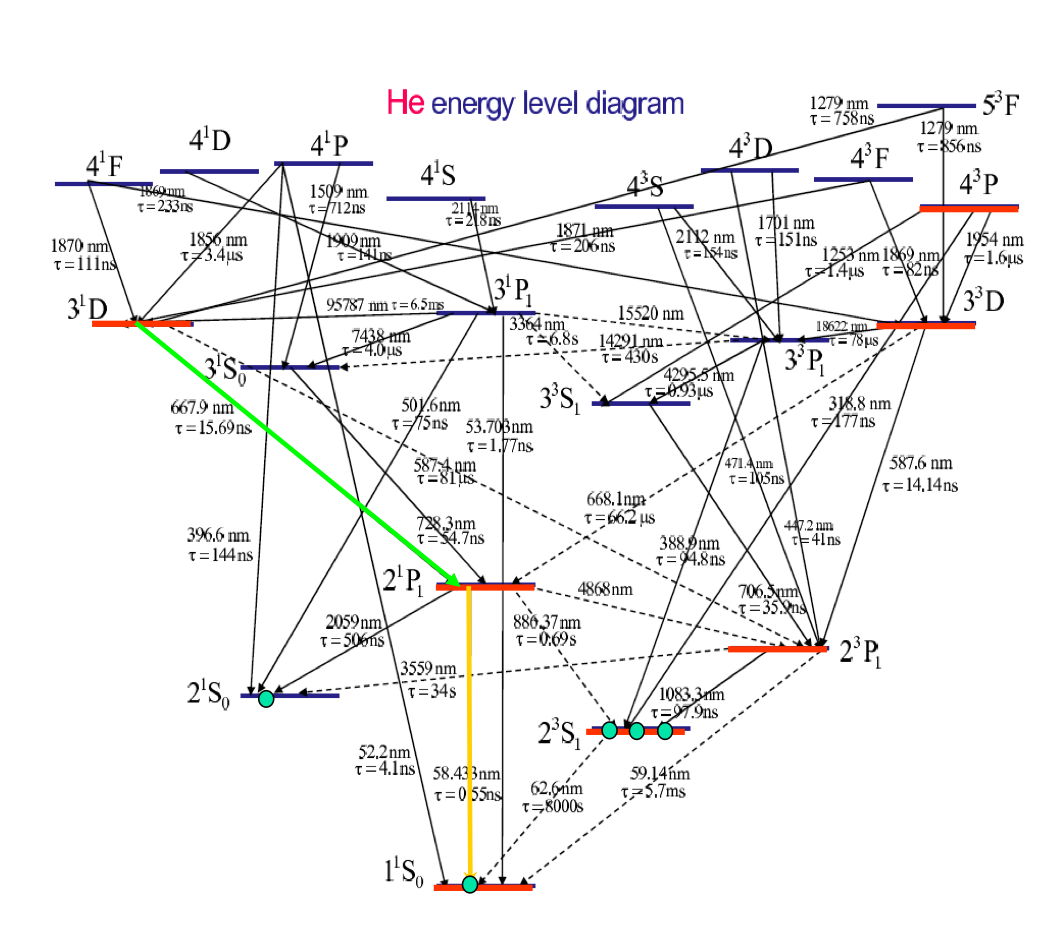
\includegraphics[width=0.9\linewidth]{ch-theory/figures/Helium_energy_levels}
    \caption[Sample Title Page Layout]{Helium energy levels~\cite{drake2007multiplet}}
    \label{fig:theory:HeEnergyLevel}
  \end{center}
\end{figure}



\chapter{Experiment\label{ch:experiment}}
\section{Apparatus}
Lasing system with a Ti:Sapphire amplifier lasing @ $800nm$, with a
pulse duration of $50ns$ and output energy of $3mJ$.

Optical parametric amplifier with a tunable wavelength wavelength
between $500nm ~ 2\mu m$, max energy is $100mJ$.
\section{Population probing techniques}
\subsection{Emission}
The first thing we want to study is probing the population at
different stages of ionized Helium. When you ionize Helium, the
electrons will recombine, cascaded down through collision to lower
state. So we want to know populations of certain level at certain
stage.

Several techniques have been developed to observe the behavior of this
ionized Helium.

The intense ionizing beam which is $800nm$ is focused to generate
ionized Helium and a plasma.
picture.

One of the emission lines of Helium which is dominating in visible, is
$587nm$.

Quantum weighs of triplet are 3 times bigger than singlet, so even the
A and B coefficient are similar, we see stronger lines.

Pressure broadening:
This is emission line at different pressure. The higher pressure you
have , the broader line width you will get.

Gated CCD spectra:
you record the spectra at different time of the Helium ionization, so
you get the dynamics of the emission of 587 lines, as a function of
time. From the spectrum, we could see that the peak occurs roughly at
$10ns$ after ionization. Besides, the width of the spectra is
shrinking as time goes by. The reason is that, after the ionization,
the density of the electron is high, and the width is due to collision
between electrons and atoms. As the plasma expand, you can see the
line gets narrower.

At different delay time, you can see different width of the spectra line.
\subsection{Transmission study}
Another technique is also developed to observe the population at
certain levels, by sending in a femto-second laser pulse, resonating
with one of the transitions.

One of the advantage of using femto-second laser is that it has very
wide spectrum, much wider than the transition itself.

So you could see absorption directly at the transmission spectra, of
the transmitted probe beam.

\subsection{Absorption vs Delay}
Typical spectra of femto-second pulse without ionizing Helium are 50fs
wide. As the time progress, you can see bigger and bigger effects of
the absorptio due to the accumulation of population of $2^3S$ over
time. This is done at fixed pressure.

\subsection{Absorption vs probe energy}
At different probing energy, you can see saturation effects because
depletion of population.

\subsection{linewidth as a function of pressure}
Another transition at $587nm$, which you also see this absorption
effects, we can carefully measure the line width at different
pressure.

Low pressure, it's linear, at higher pressure, because of saturation,
it's non-linear.

We have developed a method for probing the population evolution of
excited atoms, we are going to use this not only to measure the
population, but also linewidth, such as collision rates.

\section{Broadening Analysis}
Experiments show the line broadening of $587nm$ ($2^3P->3^3D$) is
$0.5nm$, while $1080nm$ ($2^3s->2^3P$), it's $0.4nm$

The Experiment Parameters are:
Helium: $200mbar$, the atom density is $5x10^{18}cm^{-3}$
Probe beam delay: $10ns$
Electron density: $2x10^{17}cm^{-3}$
Atom density(excited): $10^{14}cm^{-3}$
Electron temperature: $0.5eV$

For a rough estimation of electron-atom collision cross section, we
could use the equation as follows:
\begin{equation}
\sigma_{ea} = (n^2a_B)^2; \tau_{ea}=\frac{1}{N_e v_e \sigma_{ea}} =
212 ps (for 1.08 \mu m)
\end{equation}
picture.

There are different broadening mechanism:
- Natural: quite narrow, usually on the order of $1/1000$ $\Delta
\lambda_{collision}$, so could be neglected.
- Doppler: Due to thermal motion of the emitter.
- Instrumental: Equals to slit width times dispersion by grating.
- Collisional: When emitting, if the emitter colloided by other
particles, the emitting process will be disturbed.
- Other: Like the superradiance?

\subsection{Doppler Broadening}
\begin{equation}
\Delta w = 2 \sqrt{ln2} \sqrt{ \frac{2kT \lambda^2_0}{mc^2} }
\end{equation}

For $587nm$: $\Delta w_D = 0.32 nm$ while total is $5 \AA$.
For $1080nm$: $\Delta w_D = 0.59 nm$ while total is $24 \AA$.

So the Doppler broadening could be neglected.

\subsection{Instrumental Broadening}
Slit width: $40\mu m$

Instrumental broadening: $4 \AA$

Subtract instrumental from total:

587: $\sqrt{0.5^2-0.4^2} = 0.3 nm ~ 2.1 ps$

1080: $\sqrt{2.4^2-0.4^2} = 2.36 nm ~ 0.6 ps$

\subsection{Collisional Broadening}
Picture.

There's atom-atom collision and atom-election collision
(?electron-electron?)

But since the electron density ($10^{17}cm^{-3}$) is much higher than
atom density ($10^{14}cm^{-3}$), so the electron-atom collision will
dominate.

The weight of atoms are much higher than electrons, so atoms could not
gain much speed when laser present, while electron is fast!

Electron atom collision includes electron-impact excitation and
ionization, and their reverse processes, so one only need to consider
one of those processes.

Our electron is cold, only $0.5eV$, so the ionization cross section is
small, which could be neglected.

After the laser passed, it could be assumed that there's no photon, so
all photon related process like photo ionization/excitation could be
neglected.

Our electron density is high $10^{17}cm^{-3}$, so after laser passed,
electron reaches their local thermal equilibrium (LTE)(ref) quickly, at
$10ns$. Of course, Maxwellian distribution could be assumed.

To summarize, we just need to consider electron impact excitation,
under electron Maxwellian distribution.

From the Ralchenko paper(ref), we found the cross section fitting
curve, for electron impact transition between different states. This
curve is trustable, for it match experiments quite well.

The cross section is given by:
\begin{equation}
\sigma(E,\Delta E) = a_0^2 \pi \frac{R_y}{g_l E}
\Omega(\frac{E}{\Delta E})
\end{equation}
Where $a_0$ is just Bohr radius, $\pi a_0^2 = 0.8797 * 10^{-16} cm^2$,
$g_l$ is the statistical weight, for $2^3 S$ and $2^3 P$, $g_l = 3$.
$R_y = 13.6057 eV$ is the Rydberg energy. And $E$ is the collisional
energy, where $E=\frac{1}{2}mv^2$, $v$ could be calculated by
averaging through a Maxwellian distribution.

picture.

$\Delta E$ is the energy difference between initial and final states,
for $587nm$: it's $\frac{1.24}{0.587} eV$, while for $1080nm$, it's
$\frac{1.24}{1.08} eV$.

\begin{equation}
\Omega(x) = (A_1 ln(x) + A_2 + \frac{A_3}{x} + \frac{A_4}{x^2} +
\frac{A_5}{x^3}) (\frac{x+1}{x+A_6})
\end{equation}

For $2^3S -> 2^3P$, those coefficients are:

\begin{tabular}{ l | r }
  $A_1$ & $7.696 * 10^1$ \\
  $A_2$ & $1.250 * 10^2$ \\
  $A_3$ & $4.938 * 10^1$ \\
  $A_4$ & $-4.778 * 10^1$ \\
  $A_5$ & $3.189 * 10^2$ \\
  $A_6$ & $8.157$
\end{tabular}

While for $2^3S -> 2^3P$, those coefficients are:

\begin{tabular}{ l | r }
  $A_1$ & $1.414 * 10^2$ \\
  $A_2$ & $9.031 * 10^1$ \\
  $A_3$ & $-6.238 * 10^2$ \\
  $A_4$ & $1.183 * 10^3$ \\
  $A_5$ & $-6.424 * 10^2$ \\
  $A_6$ & $8.626$
\end{tabular}

So now we got everything to estimate $\sigma v$
\begin{equation}
\sigma(E,\Delta E) = \pi a_0^2 \frac{R_y}{g_l E}\Omega(\frac{E}{\Delta
E})
\end{equation}

Since we have Maxwellian distribution:
\begin{equation}
f(v) dv = (\frac{m}{2\pi k T})^(\frac{3}{2})4\pi v^2
exp(\frac{-mv^2}{2kT}) dv
\end{equation}

by switching to energy using, $E=\frac{1}{2}mv^2$, $v=\sqrt{2E}{m}, dv
=\frac{1}{\sqrt{2mE}}dE$, we got:
\begin{equation}
f(E)dE=(\frac{m}{2\pi k T})^{\frac{3}{2}}4\pi \frac{2E}{m} exp(-
\frac{E}{kT}) \frac{1}{\sqrt{2mE}} dE
\end{equation}
So we get:
\begin{equation}
<\sigma v> = \int_0^{+\inf} \sigma(E)\sqrt{\frac{2E}{m}}f(E)dE
\end{equation}
Then using,
\begin{equation}
\tau_{ea} = \frac{1}{N_e<\sigma v>}
\end{equation}
Where $N_e=2*10^{17}cm^{-3}$

By using Mathematica to compute the integral, it turns out that
$\tau_{ea}$ is quite small. This results is reasonable, for our
electron is cold, $kT=0.5eV$, this is small compared to $3^3D$ ->
$2^3P$ and $2^3P$ -> $2^3S$ gap, so the cross section should be small.

Picture.

However this is not the end of the story, this small result enlightens
us to focus on the electron-impact transition, whose cross section is
big in our case. Apparently, the smaller the energy difference,
between the initial and final state, the easier to excite, so the
cross section is bigger.

The total cross section is the sum of all the transitions, so let's
focus on the dominating one first.

For final state $3^3D$, the most close energy level is $3^1D$, and for
$2^3P$, it's $2^1P$. Now we look for the cross section of these two
transitions.

From graph 15 on page 617, $2^3P$ -> $2^1P$, cross section reads
$\sigma = 10^{-15}cm^2$ @ $0.5eV$

around $0.5eV$, the curve is flat enough to avoid taking average from
Maxwellian distribution.
\begin{equation*}
<v> = 2*10^7 cm/s
\end{equation*}
\begin{equation*}
<\sigma v> = \sigma <v>
\end{equation*}
\begin{equation}
\tau_{ea} = \frac{1}{N_e<\sigma v>} = \frac{1}{N_e \sigma <v>}
=\frac{1}{2*10^{17}cm^{-3}*10^{-15}cm^2*2*10^7cm/s} = 250 ps
\end{equation}

Similarly, by graph 28 on page 619, we found excitation from $3^3D$ ->
$3^1D$ dominates, whose cross section reads:
\begin{equation}
\sigma = 4.5 * 10^{-15} cm^2
\tau_{ea} = \frac{1}{N_e\sigma<v>} = 55ps
\end{equation}

But this could not explain all the broadening from experiments:

\begin{tabular}{ l c r }
       & Experiment & Calculation \\
  587  & 0.3nm(2.1ps) & 55ps \\
  1080 & 2.2nm(0.6ps) & 250ps \\
\end{tabular}

This indicates, there should be broadening factors brought in by other
effects. It should be superradiance. In that case, only the cylinder
of atoms contributes to superradiance, whose radius is $\lambda$, and
the length is plasma length.

Picture.

For 587nm, the single atom decay is given by:
\begin{equation}
\tau = \frac{1}{A} = 14ns
\end{equation}
The superradiance factor is:$N_a\lambda^2L/2\pi$, where
$N_a=10^{14}cm^{-3}$, $\lambda=587nm$, $L=0.7cm$, so the broadening
brought in by superradiance is:
\begin{equation}
\tau_s=\frac{\tau}{N_a\lambda^2L/2\pi} \\
= \frac{14ns}{10^{14}*0.587^2*10^{-8}*0.7/2\pi} = 0.364ps
\end{equation}
compared with $0.3ps$ experimental measurements, they are on the same
order.

For $1080nm$, $N_a$ is larger, and
\begin{equation}
\tau=\frac{1}{A}=100ns
\end{equation}
\begin{equation}
\tau_s=\frac{\tau}{N_a\lambda^2L/2\pi}=\frac{100ns}{4*10^{14}*1.08^2*0.7*10^{-8}/2\pi}=0.192ps
\end{equation}
While the width measured from experiment is $0.2ps$, they are on the
same order.

\section{Simulation Results}
If after ionization, a Maxwellian distribution could be assumed, it
will be quite handy. For only two parameters are needed to describe
the whole system. Otherwise, a more complicated method need to be take
to handle the distribution, like the code we are using, which traces
all the particles one by one.


\section{Superradiance}
\section{Carbon line identification}
%\section{Preliminary data and results on emission and absorption by excited Helium atoms}


%\section{Options}
\label{sec:usage:options}

In this section, we describe the options you can set when using this thesis class.
\tablespacing
% tablespacing is defined by the class to set single spacing for the long table when in doublespacing mode. If the singlespace option is set, this command has no effect.

\begin{longtable}{p{0.3\linewidth} p{0.6\linewidth}}

  % First page heading
  \caption[Options Provided by the PUthesis Class]{List of options for the puthesis document class and template} \label{tab:usage:options}\\
  \toprule
  \textbf{Option} & \textbf{Description} \\
  \midrule
  \endfirsthead

  % Future page heading
  \caption[]{(continued)}\\
  \toprule
  \textbf{Option} & \textbf{Description} \\
  \midrule
  \endhead

  % Page footer
  \midrule
  \multicolumn{2}{r}{(Continued on next page)}\\
  \endfoot

  % Last page footer
  \bottomrule
  \endlastfoot

  12pt &
  Specify the font size for body text as a parameter to \texttt{documentclass}. The Mudd Library requirements~\cite{muddthesis2009} state that 12pt is preferred for serif fonts (e.g., Times New Roman) and 10pt for sans-serif fonts (e.g., Arial).
  \\

  letterpaper &
  If your document is coming out in a4paper, your LaTeX defaults may be wrong. Set this option as a parameter to \texttt{documentclass} to have the correct 8.5"x11" paper size.
  \\

  lot &
  Set this option as a parameter to \texttt{documentclass} to insert a List of Tables after the Table of Contents.
  \\


  lof &
  Set this option as a parameter to \texttt{documentclass} to insert a List of Figures after the Table of Contents and the List of Figures.
  \\

  los &
  Set this option as a parameter to \texttt{documentclass} to insert a List of Symbols after the Table of Contents and the other lists.
  \\

  singlespace &
  Set this option as a parameter to \texttt{documentclass} to single space your document. Double spacing is the default otherwise, and is required for the electronic copy you submit to ProQuest. Single spacing is permitted for the printed and bound copies for Mudd Library.
  \\
  
  draft &
  Set this option as a parameter to \texttt{documentclass} to have \LaTeX mark sections of your document that have formatting errors (e.g., overfull hboxes). 
  \\

  % the cmidrule here spans both columns but is indented slightly on the left and right. 
  \cmidrule[0.1pt](l{0.5em}r{0.5em}){1-2}

  \raggedright
  $\backslash newcommand$ $\{\backslash printmode\}\{\}$ &
  Insert this command after the \texttt{documentclass} command to turn off the hyperref package to produce a PDF suitable for printing.
  \\

  \raggedright
  $\backslash newcommand$ $\{\backslash proquestmode\}\{\}$  &
  Insert this command after the \texttt{documentclass} command to turn off the `colorlinks' option to the hyperref package. Links in the pdf document will then be outlined in color instead of having the text itself be colored. This is more suitable when the PDF may be viewed online or printed by the reader.
  \\

  $\backslash makefrontmatter$ &
  Insert this command after the \texttt{$\backslash begin\{document\}$} command, but before including your chapters to insert the Table of Contents and other front matter.
  \\
  
  \cmidrule[0.1pt](l{0.5em}r{0.5em}){1-2}

  $\backslash title$ &
  Set the title of your dissertation. Used on the title page and in the PDF properties.
  \\

  $\backslash submitted$ &
  Set the submission date of your dissertation. Used on the title page. This should be the month and year when your degree will be conferred, generally only January, April, June, September, or November. Check the Mudd Library rules~\cite{mudd2009} for the appropriate deadlines.
  \\

  $\backslash copyrightyear$ &
  Set the submission year of your dissertation. Used on the copyright page.
  \\

  $\backslash author$ &
  Your full name. Used on the title page, copyright page, and the PDF properties. \\

  $\backslash adviser$ &
  Your adviser's full name. Used on the title page. \\

  $\backslash departmentprefix$ &
  The wording that precedes your department or program name. Used on the title page. The default is ``Department of'', since most people list their department and can leave this out (e.g., Department of Electrical Engineering), however if yours is a program, set $\backslash departmentprefix\{Program in\}$ \\

  $\backslash department$ &
  The name of your department or program. Used on the title page. \\

  \cmidrule[0.1pt](l{0.5em}r{0.5em}){1-2}
  
  \raggedright  
  $\backslash renewcommand$ $\{\backslash maketitlepage\}\{\}$ &
  Disable the insertion of the title page in the front matter. This is useful for early drafts of your dissertation. \\

  \raggedright  % full justification places the * in an awkward place
  $\backslash renewcommand*\{\backslash makecopyrightpage\}\{\}$ &
  Disable the insertion of the copyright page in the front matter. This is useful for early drafts of your dissertation. \\

  \raggedright 
  $\backslash renewcommand*\{\backslash makeabstract\}\{\}$ &
  Disable the insertion of the abstract in the front matter. This is useful for early drafts of your dissertation. \\

\end{longtable}
\bodyspacing
% bodyspacing restores double spacing or single spacing after the table

% need blank space after \bodyspacing

I've seen other people print their dissertations using $\backslash pagestyle\{headings\}$, which places running headings on the top of each page with the chapter number, chapter name, and page number. This documentclass is not currently compatible with this option -- the margins are setup to be correct with page numbers in the footer, placing them 3/4" from the edge of the paper, as required. If you wish to use headings, you will need to adjust the margins accordingly.






\chapter{Conclusion\label{ch:conclusion}}

In this work, we explain how to use the puthesis.cls class file and the accompanying template.   % Conclusion
\section{Future Work}

Future work should include options in the template for a masters thesis or an undergraduate senior thesis. It should also support running headings in the headers using the `headings' pagestyle.  The print mode and proquest mode included in the template might also be candidates to include in the class itself. 

  % Future work

\appendix % all chapters following will be labeled as appendices
\chapter{Implementation Details\label{ch:implementation}}

Appendices are just chapters, included after the $\backslash appendix$ command.

\section{Switching Formats}
When switching \texttt{printmode} on and off (see Section~\ref{sec:usage:options}), you may need to delete the output .aux files to get the document code to compile correctly. This is because the hyperref package is switched off for \texttt{printmode}, but this package inserts extra tags into the contents lines in the auxiliary files for PDF links, and these can cause errors when the package is not used.

\section{Long Tables}

Long tables span multiple pages. By default they are treated like body text, but we want them to be single spaced all the time. The class therefore defines a new command, $\backslash tablespacing$, that is placed before a long table to switch to single spacing when the rest of the document is in double spacing mode. Another command, $\backslash bodyspacing$, is placed after the long table to switch back to double spacing. Normal tables using \texttt{tabular} automatically use single spacing and do not require the extra commands.

When the documentclass is defined with the `singlespace' option, these commands are automatically adjusted to stay in single spacing after the long table.

Make sure there is always at least one blank line after the $\backslash bodyspacing$ command before the end of the file.

Some times long tables do not format correctly on the first pass. If the column widths are wrong, try running the \LaTeX compiler one or two extra times to allow it to better calculate the column widths.

If you want your long table to break pages at a specific point, you can insert the command $\backslash pagebreak[4]$, to tell \LaTeX that it really should put a page break there. $\backslash pagebreak[2]$ gives it a hint that this is a good place for a page break, if needed. If there's a row that really should not be broken across a page, use $\backslash \backslash *$, which will usually prevent a pagebreak. 

\section{Booktabs}
The booktabs package is included to print nicer tables. See the package documentation~\cite{fear2005booktabs} for more details and motivation. Generally, all vertical lines are removed from the tables for a better visual appearance (so don't put them in), and better spacing and line thicknesses are used for the horizontal rules. The rules are defined as $\backslash toprule$ at the top of the table, $\backslash midrule$ in between the heading and the body of the table (or between sections of the table), and $\backslash bottomrule$ at the end of the table. $\backslash cmidrule$ can be used with the appropriate options to have a rule that spans only certain columns of the table.

\section{Bibliography and Footnotes}

The bibliography and any footnotes can also be single spaced, even for the electronic copy. The template is already setup to do this.

Bibliography entries go in the .bib file. As usual, be sure to compile the \LaTeX code, then run BibTeX, and then run \LaTeX again.

To cite websites and other electronically accessed materials, you can use the `@electronic' type of BibTeX entry, and use the `howpublished' field to include the URL of the source material.

The formatting of bibliography entries will be done automatically. Usually the titles are changed to have only the first word capitalized. If you'd prefer to have your original formatting preserved, place the title in an extra set of curly braces, i.e., ``title = \{\{My title has an AcroNyM that should stay unchanged\}\},''.

\section{Figures and Tables}
The captions of figures and tables take an optional parameter in square brackets, specifying the caption text to be used in the Table of Contents. The regular caption in curly braces is used for the table itself.

Generally captions for tables are placed above the table, while captions for figures are placed below the figure.




%\chapter{Printing and Binding\label{ch:printing}}

\section{Printing}

For the library copies of your dissertation, you must use archival quality printing and binding. This means acid-free paper, containing at least 25\% cotton fiber. Triangle Repocenter on Nassau Street in Princeton offers both 25\% cotton paper and 100\% cotton paper. Most people choose the 25\% cotton paper, and this is generally recommended by the binders. The 100\% copy paper is somewhat thicker and the extra expense is unnecessary. 

Triangle offers online submission of your printing and binding order at: \url{http://triangleprinceton.com/collegiatebinding/thesis/}. If you request binding from them, they will deliver the paper copies to Smith-Shattuck Bookbinding for you and allow you to pick up the completed copies at their store on Nassau Street. The whole process takes 2-3 business days, but check with them in advance during the busy thesis-printing season in April and May. 

Currently, your printed and bound dissertation copies can be single spaced. Only the electronic copy submitted to ProQuest must be double spaced. All copies must be printed single-sided, with specific margins. 

\section{Binding}

An archival-quality sewn binding is required for the library copies of your dissertation. Smith-Shattuck Bookbinding is highly recommended, and is used by most students. Triangle Repocenter will send your copies there for you, greatly simplifying the process, but you can call Smith-Shattuck with special requests. 

The ``library standard'' sewn binding is sufficient for the copies to be sent to Mudd Library. It uses a black buckram cloth cover, which is the most popular option. For extra copies for yourself and your family members, you can choose ``buckram roundback binding'', which adds decorative lines on the spine, and printing of the title and author on the front cover. For a small additional fee, you can include the Princeton University shield on the front cover and a ribbon bookmark. Leather covers are also available. See Smith-Shattuck's website for more details at: \url{http://www.thesisbookbinding.com/}. 


%% Make the bibliography single spaced
\singlespacing
\bibliographystyle{plain}

%% add the Bibliography to the Table of Contents
\cleardoublepage
\ifdefined\phantomsection
  \phantomsection  % makes hyperref recognize this section properly for pdf link
\else
\fi
\addcontentsline{toc}{chapter}{Bibliography}

%% include your .bib file
\bibliography{lch-pums-thesis}

\end{document}

